\todo[inline]{FROM PRELIMINARY. INCORPORATE ELSEWHERE}
In this chapter, preliminary work related to the thesis is presented. This includes a convolutional neural network developed for road detection, and a dataset containing aerial images of Norwegian roads, which will be outlined in Section \ref{sec:Method}. In Section \ref{sec:Experiment} some preliminary tests are presented, and future work can be found in Section \ref{sec:Future_work}. 

\section{Method}
\label{sec:Method}
\subsection{The road extraction system}
The road extraction system was written in Python, and uses the open source library Theano. Theano enables the user to define and evaluate mathematical expressions involving tensors. The library implements several useful features for developing \ac{CNN}s, such as back-propagation, convolution, and max pooling. Training deep neural networks on a \ac{GPU} can be considerably faster than on a \ac{CPU}. Theano can utilize both the \ac{CPU} and \ac{GPU} without making any modifications to the code.\\

The system is based on the deep neural network outlined by \cite{Mnih_aerial_images_noisy}. The network have three convolutional layers and two fully connected layers. This network architecture is depicted in Figure \ref{fig:conv}. After the network is trained, it can predict whether or not roads are present in a $16 \times 16$ pixel area contained in the center of a $64 \times 64$ aerial image patch. The input patch is considerably larger than the output patch, so that the network can better utilize the context in the image. \\

The first layer perform convolution using 16x16 kernels, and outputs in total 64 feature maps. Only the first layer utilize max pooling, which reduces the number of inputs to the next layer as well as introducing some translational invariance to the model. The kernel size in the second and third layer are currently $4 \times 4$ and $3 \times 3$, respectably. The output of the third convolutional layer is used as input to a fully connected neural network with a single hidden layer and an output layer. The latter contains 256 units where each output is the probability of a pixel representing a road.\\

To avoid overfitting the training data, and hopefully achieve better generalization, different regularization schemes are applied during optimization, such as L2 weight decay, early stopping, and the dropout technique. The first applies a weight penalty to prevent weights from growing large. The second stops the optimization process when performance on the validation set starts to consistently decrease. This is an indication of the model starting to overfit the training set. Dropout forces the units to rely less on each other, by randomly disabling half of the units in the network during training. This encourage units to encode independently useful information, since dropout penalize co-adaptation between units.\\

The model parameters are optimized with a special form of \ac{SGD}, called RMSProp. RMSProp keeps a running average of the gradient magnitude for every weight which is used to adaptively adjust the learning rate of each weight. Compared to \ac{SGD}, this will result in a faster convergence. Other optimizers, such as Nesterov momentum, have also been implemented.\\

Before training occurs, a patch dataset suitable for the model is constructed. Each data and label image is rotated by a random amount, and a predefined number of image and label patches are extracted from the images. Before adding the sample to the training set, contrast normalization is applied. The mean pixel value in a patch is subtracted from each pixel, and divided by the standard deviation found for all pixels in the dataset.\\

\subsection{The Norwegian roads dataset}
\label{sec:Norwegian_roads_dataset}
In addition to the Massachusetts Roads Dataset \citep{MnihThesis}, the proposed algorithm will be tested on a new dataset. This dataset was constructed from aerial images retrieved from Kartverket, which depicts both rural and urban areas in Norway. The labels for this dataset have been generated from road center-line vectors found in the publicly available topographic vector database, N50, provided by Kartverket. \\

Currently, the dataset contains 221 RGB images that are 1536 pixels in width and height. The images have a high resolution with a \ac{GSD} of around 0.66 meters per pixel. There are 184 images in the training set, 21 images in the validation set, and 16 images in the test set. The road center-line vectors are generated as 4 pixel wide black lines in the label images. A cropped image from this dataset can be seen in Figure \ref{fig:aerialimage_norwegian}, with the label image superimposed on the aerial image. Observe that some roads are missing from the label image, as well as the ground truth not covering the roads properly. \\

\begin{figure}[t]
\begin{center}
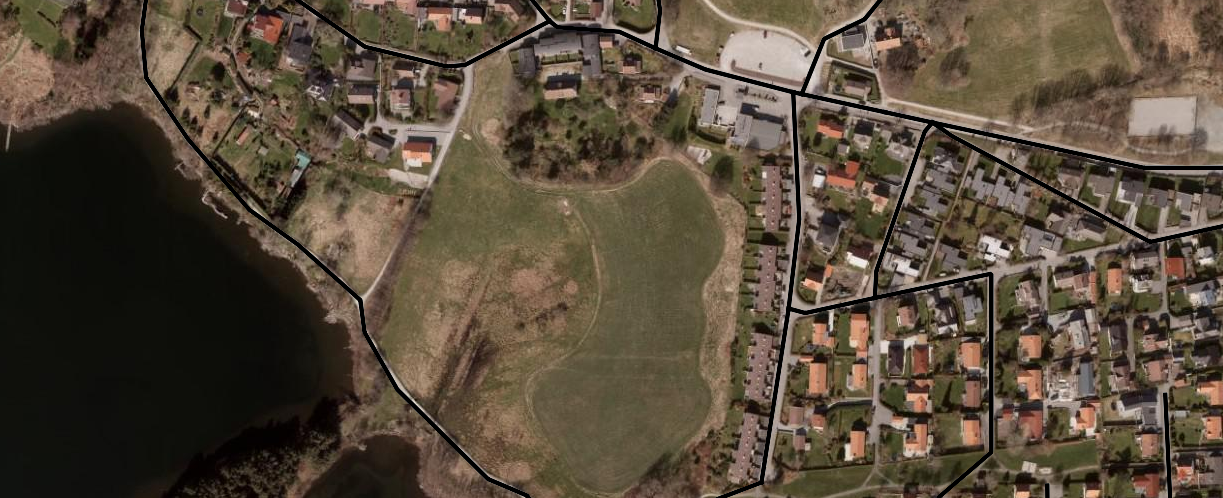
\includegraphics[width=1\columnwidth]{figs/norwegian_dataset.png}
\caption[Norwegian road dataset example]{Example aerial image with the label image as an overlay.}
\label{fig:aerialimage_norwegian}
\end{center}
\end{figure}

The Norwegian Roads Dataset has been constructed by using QGIS, an open source geographic information system application. The application enables viewing and editing of map data, but also provides a Python interface. A script to create label images was developed, which takes the map coordinates associated with each corner of an aerial image, and generates a raster image of road center-line vectors found inside that area. These raster images can be used as label data in supervised learning. \\


\section{Experiment}
\label{sec:Experiment}
The performance of the system has not been compared to \citep{saito_building_and_roads} and \citep{Mnih_aerial_images_noisy}, due to the fact that the precision and recall metrics described in Section \ref{sec:background_theory} have not been implemented yet.\\

Nonetheless, the center image in Figure \ref{fig:result} illustrates the current performance of the system. In this particular test image, the model is able to identify the majority of the roads present, except for a small gravel road on the right side of the image. There are also a lot of prediction errors, such as roads being disconnected, and prediction artefacts in the forest areas. An interesting observation is that the model also correctly predicts small private roads leading up to houses present in the image. Furthermore, the model detects construction roads in the upper left corner. Since these roads are not present in the label image, the model is penalized for these predictions by the cross-entropy loss function.\\


\begin{figure}[t]
\centering
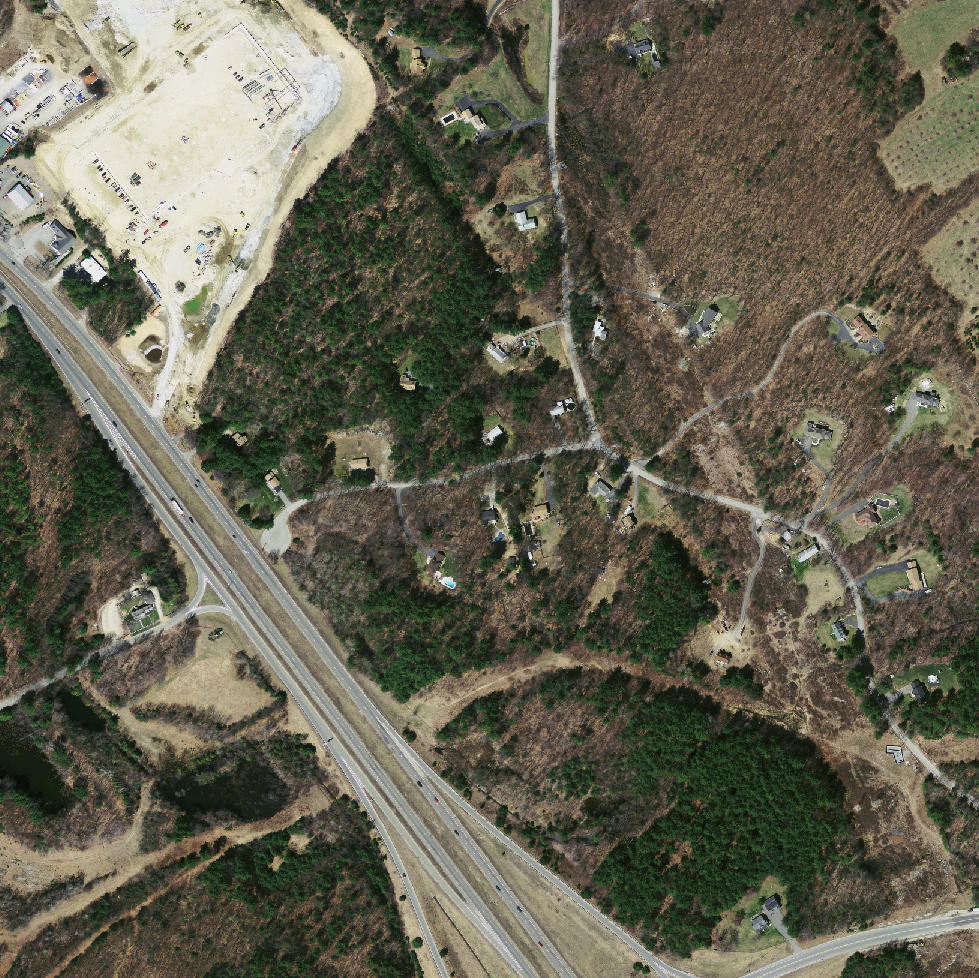
\includegraphics[width=.32\textwidth]{figs/results_data.jpg}\hfill
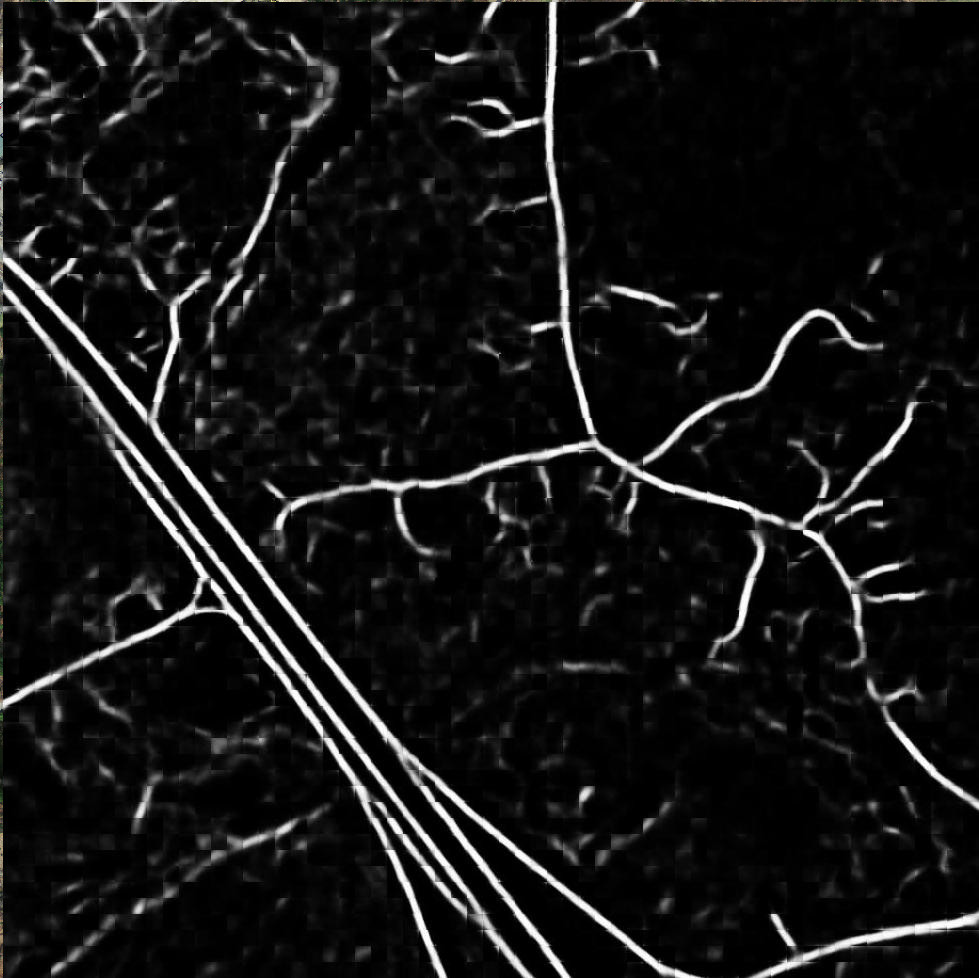
\includegraphics[width=.32\textwidth]{figs/results_label.jpg}\hfill
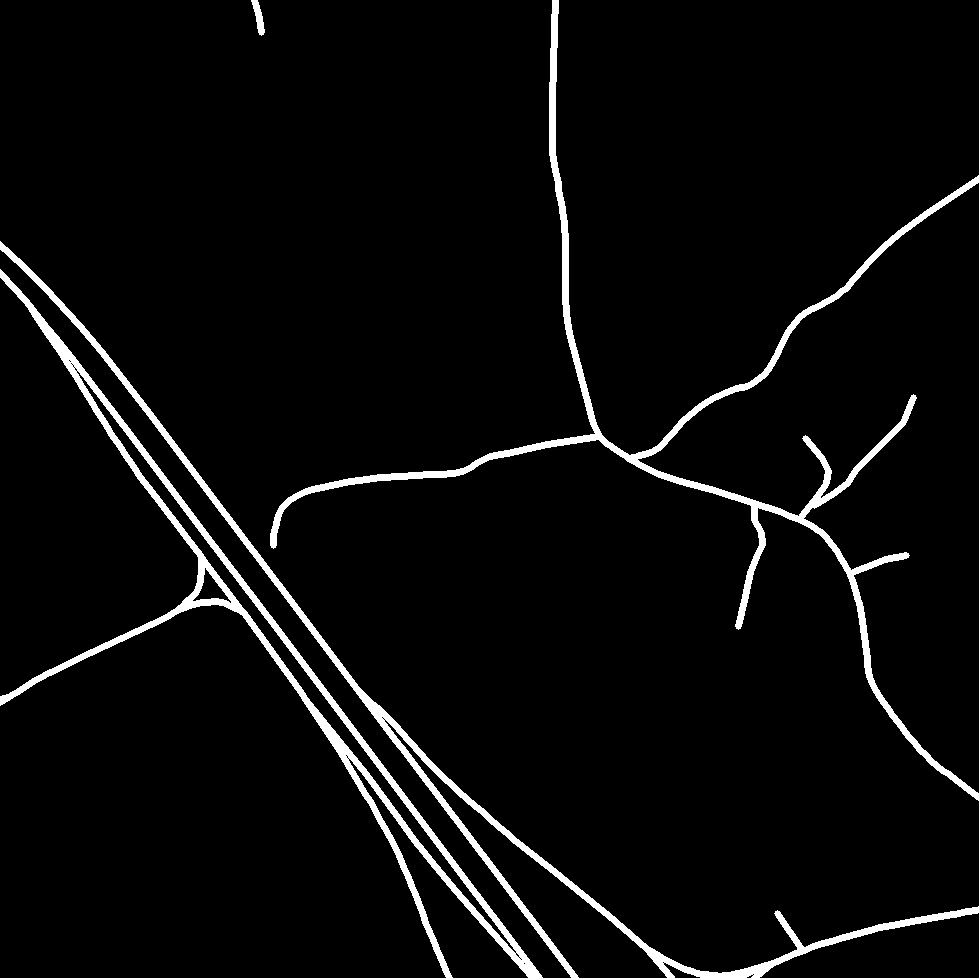
\includegraphics[width=.32\textwidth]{figs/label.png}

\caption{Aerial image, model prediction and label image. The aerial image is part of test set in Massachusetts Roads Dataset}
\label{fig:result}
\end{figure}

\section{Future work}
\label{sec:Future_work}
The current system needs to be further tested, and extensions are required in order to evaluate the research questions. For the system itself, there are two important improvements. First, the system must implement precision and recall. This enables comparisons of other similar systems created for road detection. Additionally, the system performance can be displayed using precision-recall curves. To create this type of plot, threshold operations are applied to the model prediction probabilities for different values between $0 \leq T \leq 1$. This results in values that shows the trade-off between precision and recall in the system. Second, a scheme for gradually swapping out the data on the \ac{GPU} needs to be implemented. The bottleneck for the current system is the limited size of the training set, caused by the insufficient memory size of the \ac{GPU}. Currently, the training set can only hold 30000 samples, when training on a \ac{GPU}. This is not enough for a classifier to learn the variability present in aerial images. In comparison, \cite{Mnih_roads_high_res_aerial_images} utilized 1.2 million training samples.\\

The road detection system consists of a \ac{CNN}. This was shown, by \cite{MnihThesis}, to give better performance than locally connected neural networks with untied weights. However, there are still parts of the network architecture worth exploring further. For instance, can increasing the number of convolutional layers improve the network's ability to extract features? Tweaking the kernel sizes of the different layers could also be beneficial, and if an input layer connected to a neighbourhood larger than a $64 \times 64$ pixels can better resolve ambiguous in the data. \cite{MnihThesis} also suggested adapting the loss function to maximize the area under the precision-recall curve. Furthermore, different optimization techniques, such as Nesterov momentum and RMSProp, could be compared.\\

One of the most compelling ways of improving performance for road detection, is utilizing structured output prediction methods. Several studies \citep{Kluckner_semantic_height} \citep{LeCun_semantic} \citep{Mnih_roads_high_res_aerial_images} have shown that employing a smoothness prior, by taking neighbouring predictions into account, can significantly improve generalization in semantic segmentation tasks. Implementing either \ac{CRF} or the post-processing neural network in the road detection system will therefore be considered.\\

In terms of evaluating the system, precision-recall curves will enable comparison to other systems. The system will also be trained using the Massachusetts Roads Dataset, which other road detection systems have utilized for training \citep{MnihThesis}\citep{saito_building_and_roads}. By training on the same dataset, the ability of the classifiers can more easily be compared. Furthermore, the system will also be evaluated on the Norwegian Roads Dataset. An interesting experiment would be to train the system using one of the datasets, and see what performance is achieved by the other dataset. The datasets contain two very separate areas, but also depict roads with relatively similar appearance. This might indicate how well the system captures the variability in aerial images. \\

The first research question involves reducing the effect of inconsistent labels when training a classifier. The bootstrapping approach presented by \cite{Reed_noisy_labels_bootstrapping} will be evaluated for road detection. Whereas the loss functions presented by \citep{Mnih_aerial_images_noisy} require a noise distribution model,  bootstrapping utilize a   convex combination between the classifier's prediction and the label. This approach seems to be more generally applicable, and has been tested for different tasks.\\

 An interesting improvement to this approach is to learn a time-dependent parameter for how much the classifier's own prediction should be trusted. The parameter should, at the start of training, weight the convex combination more in favor of the label. While in later stages of training, the parameter can favor the classifier's predictions more, because they have become more accurate.\\

It is important to demonstrate that the approach offers robustness to different amounts of label noise. This can be done by artificially introducing label noise in samples of road detection datasets. Omission noise can be simulated by removing a fraction of the ground truth in the label images, while registration noise can be introduced by shifting subsets of label images by a certain amount of pixels. Classifiers with the bootstrapping extension can be trained on these modified datasets, and compared to the performance achieved from baseline classifiers. The performances can then be compared at different noise levels, and reveal whether or not the technique offers any robustness towards noisy labels. Similar experiments have been conducted by \citep{Sukhbaatar_noisy_network_learning} and \citep{Reed_noisy_labels_bootstrapping} for a variety of datasets. \\

The second research question will investigate what effect a curriculum strategy can have on the road detection system's precision and recall. An interesting curriculum strategy, mentioned by \cite{Bengio_curriculumlearning}, is creating an easy-to-hard ordering of samples according to how noisy the samples are. This particular curriculum strategy might assist the bootstrapping technique, as well as being applicable for datasets containing images. A classifier is trained to a decent level for road detection, and in turn, is used to create a simple and complex dataset. Samples that are confidently and correctly predicted are considered easy and put in the simple dataset. The samples that are confidently predicted, but wrong, are assumed to be inconsistent, and therefore put in the complex dataset. The inconsistent examples will then have a higher probability of being presented later in the training procedure, when the model predictions have become more trustworthy. The convex combination of the bootstrapping approach can then be tuned more in favor of the predictions, which might avoid the negative consequences of inconsistent labelling.  It could be interesting to determine whether this curriculum strategy is beneficial for the bootstrapping technique in any way.\\

A curriculum strategy could also be defined based on image characteristics. For instance, aerial images of remote areas generally presents less complexity and ambiguity. However, this would be a more problem-specific strategy. \\ 

Alternatively, the \ac{SPL} or the \ac{SPLD} method \citep{Kumar_self_paced_learning} \citep{Lu_self-paced_learning_diversity} can be implemented in the road detection system. These methods have the advantage of not being problem-specific. In addition, the model controls the pace of learning, and there is no need to construct a fixed sequence of samples beforehand. These methods have also been evaluated for real-world datasets, and seem to work well for images. \\ 

To evaluate curriculum learning, the road detection system could be trained, using both an unaltered training scheme and with a curriculum strategy. The results can then be compared, in order to determine whether curriculum learning can achieve better generalization for road detection.\\


In summary, the loss function of the road detection system will be modified, and an alternative training regime will be used for training. To measure the effect of these modifications, the system will be compared to a baseline system, and previous results achieved by similar systems.
